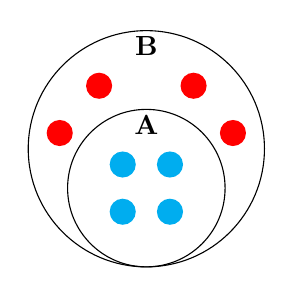
\begin{tikzpicture}
	\draw (0,0) circle (1cm);
	\draw (0,0.8) node {\textbf{A}};
	\draw (0,0.5) circle (1.5cm);
	\draw (0,1.8) node {\textbf{B}};
	
	\draw ( 0.3,  0.3) node[fill, cyan, circle] (a1) {};
	\draw ( 0.3, -0.3) node[fill, cyan, circle] (a2) {};
	\draw (-0.3,  0.3) node[fill, cyan, circle] (a3) {};
	\draw (-0.3, -0.3) node[fill, cyan, circle] (a4) {};
	
	\draw ( 1.1,  0.7) node[fill, red, circle] {};
	\draw ( 0.6,  1.3) node[fill, red, circle] {};
	\draw (-1.1,  0.7) node[fill, red, circle] {};
	\draw ( -0.6, 1.3) node[fill, red, circle] {};
\end{tikzpicture}